\section{Preliminary: Cold-start LLMs for Long Chain-of-Thought}
First, we validate whether LLMs exhibit valid Long CoT trajectories suitable for Long CoT learning. We investigate three data sources: distillation from strong reasoning LLMs, distillation from weak instruction LLMs with in-context learning (ICL), and fine-tuning on human reasoning traces.\vspace{-5pt}


\begin{figure*}[t]
    \centering
    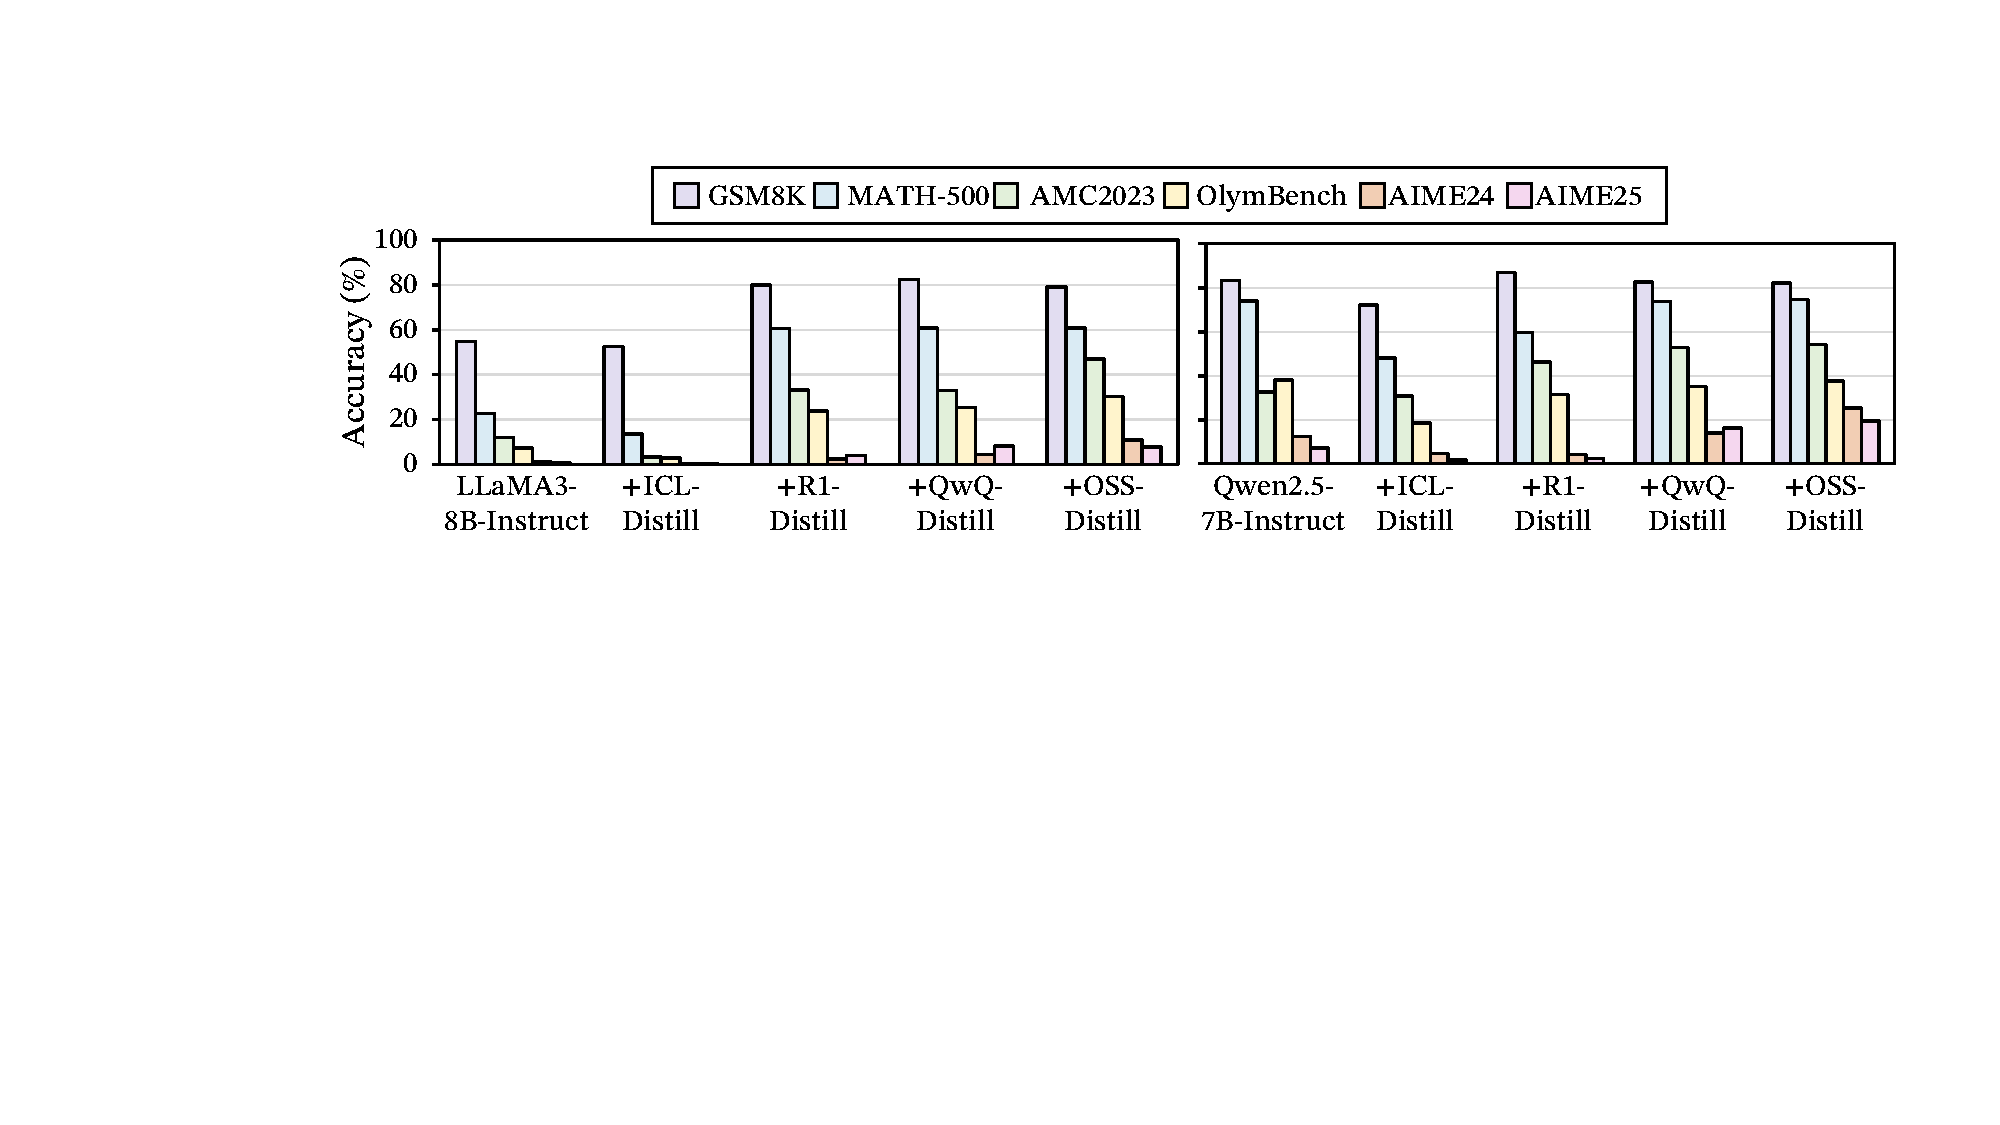
\includegraphics[width=0.96\textwidth]{figures/comparison.pdf}
    
    \caption{The failure of distillation from weak instruction LLMs with ICL and Human-annotated reasoning traces to acquire Long CoT structures, compared to successful distillation from strong reasoning LLMs. See Appendix Figure~\ref{fig:comparison-full} for the full result.}
    
    \label{fig:comparison}
\end{figure*}
\begin{wrapfigure}{r}{0.47\textwidth}
    \centering
    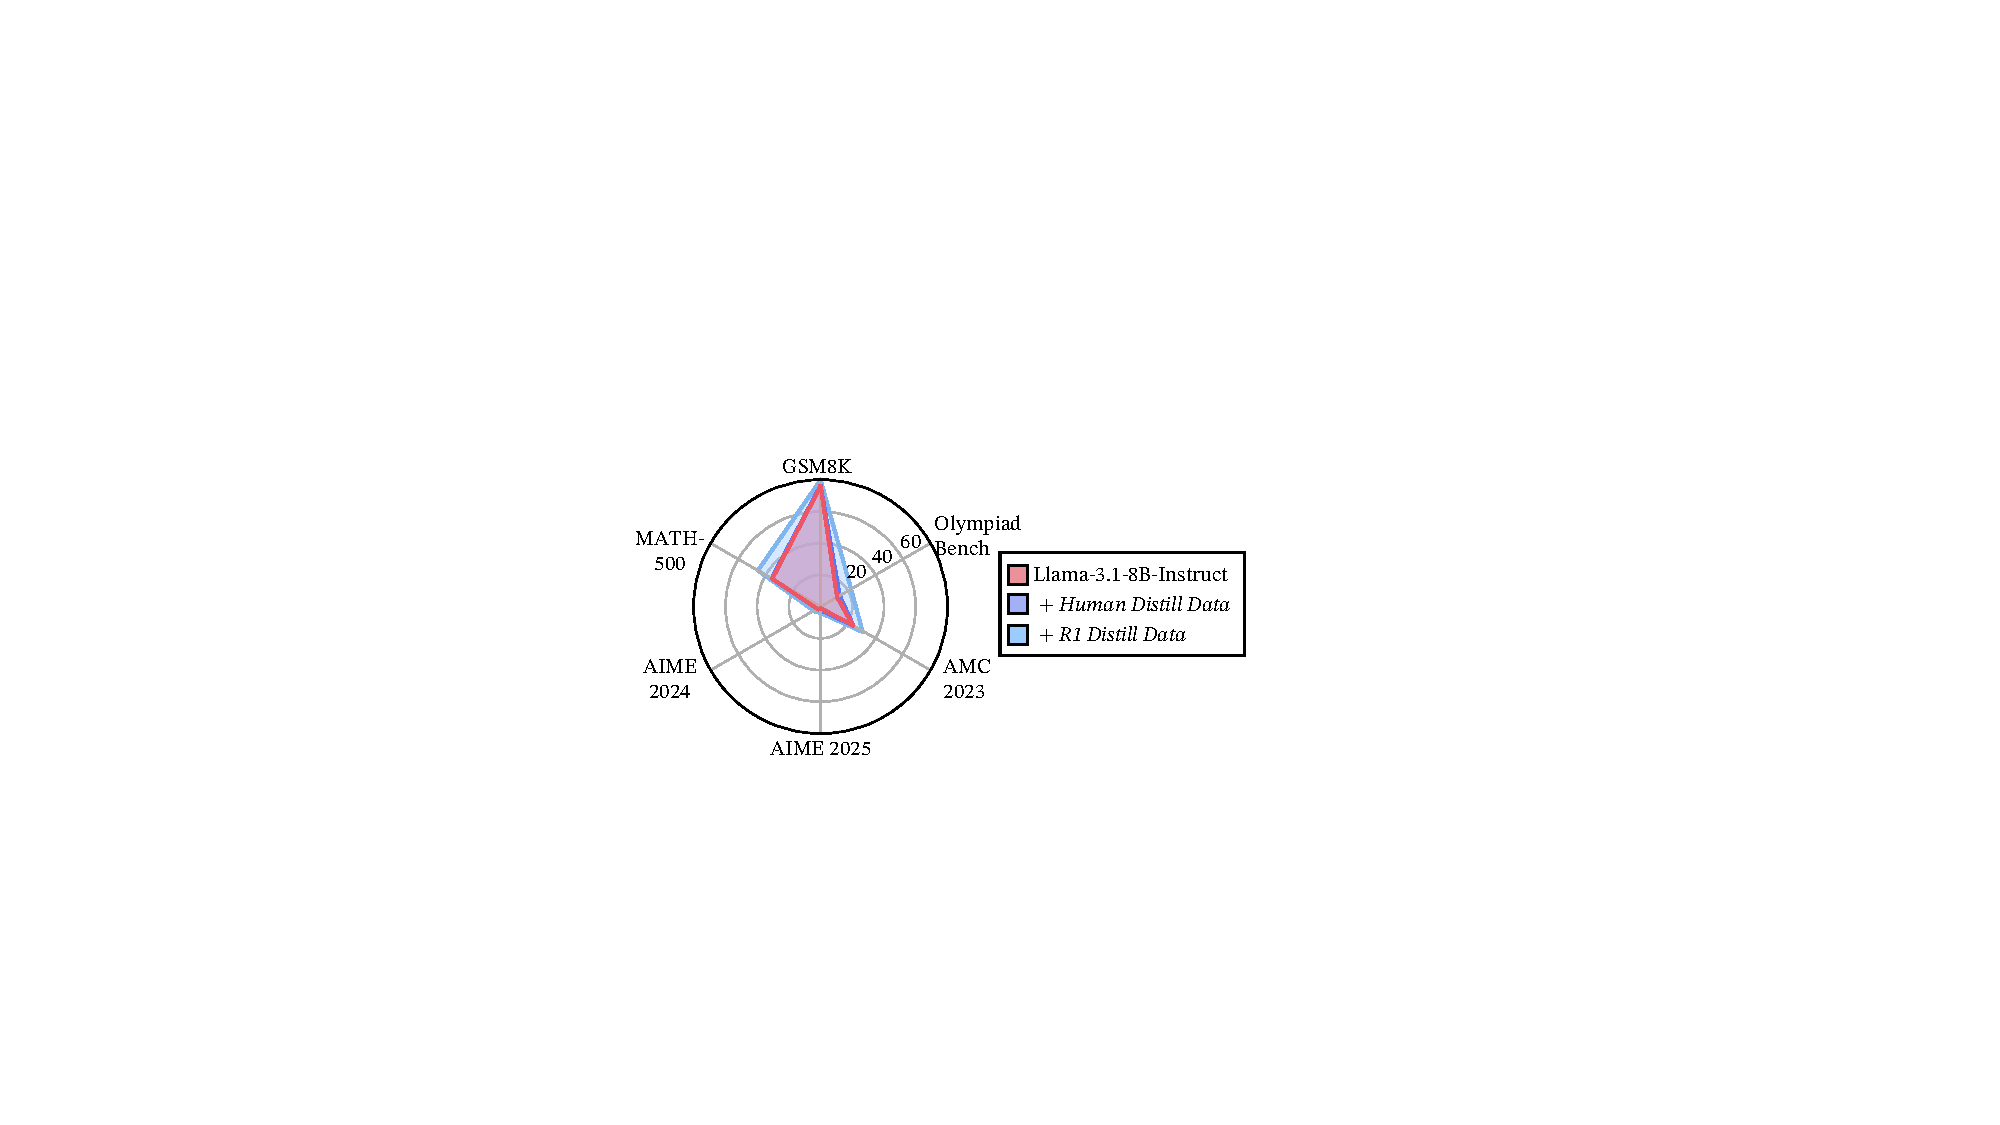
\includegraphics[width=0.46\textwidth]{figures/human.pdf}
    \caption{Performance comparison between human-annotated reasoning traces (\textit{+ Human Distill Data}) and R1 distilled reasoning traces (\textit{+ R1 Distill Data}).}
    \label{fig:human}
    \vspace{-5pt}
\end{wrapfigure}

\paragraph{\textbf{Only distillation from strong reasoning LLMs works.}}
To identify effective data sources, we curated a synthetic set of reasoning traces from three sources. As shown in Figure~\ref{fig:comparison}, only distillation from strong reasoning LLMs enables target models to learn and retain Long CoT structure, improving performance on benchmarks requiring extended reasoning. These results indicate that only high-quality traces reliably support both learning and use of Long CoT structures.\vspace{-8pt}




\paragraph{\textbf{Distillation from randomly selected ICL by weak instruct LLMs does not work.}}
Instruction LLMs without explicit reasoning training lag behind reasoning-specialized models. We test whether LLMs can acquire Long CoT structure by distilling from an instruction LLM using randomly selected ICL demonstrations that emulate Long CoT reasoning. As shown in Figure~\ref{fig:comparison}, performance drops sharply. Instruction LLMs can only mimic short CoT traces ($\thicksim$6–8 steps) and fail to extend exploration while preserving intermediate steps and trace coherence. This degradation indicates a limitation of ICL-based distillation rather than robust long-chain imitation.\vspace{-8pt}


\paragraph{\textbf{Even human-annotated Long-CoT-like traces fail.}}
Inspired by \citet{du2025the}, we test whether human step-by-step solutions can induce long CoT. We collect human solutions for complex reasoning tasks and fine-tune LLMs on them. Figure~\ref{fig:human} shows that human-trace training does not reproduce the long-CoT gains from distilling strong reasoning models, suggesting that human solutions aid local problem solving but may not reliably encode abstractions for long-horizon reasoning distributions.

\begin{TakeawayBox}{Takeaway 1}
Distillation from strong reasoning LLMs effectively imparts long CoT structures, while ICL from weak instruction models and fine-tuning on human traces yield limited gains. This underscores the importance of high-quality reasoning exemplars for robust long-chain learning in LLMs.
\end{TakeawayBox}